%!TEX root = ../surface_reconstruction.tex


\section{Описание последовательно алгоритма}
Здесь будет описание последовательного алгоритма  

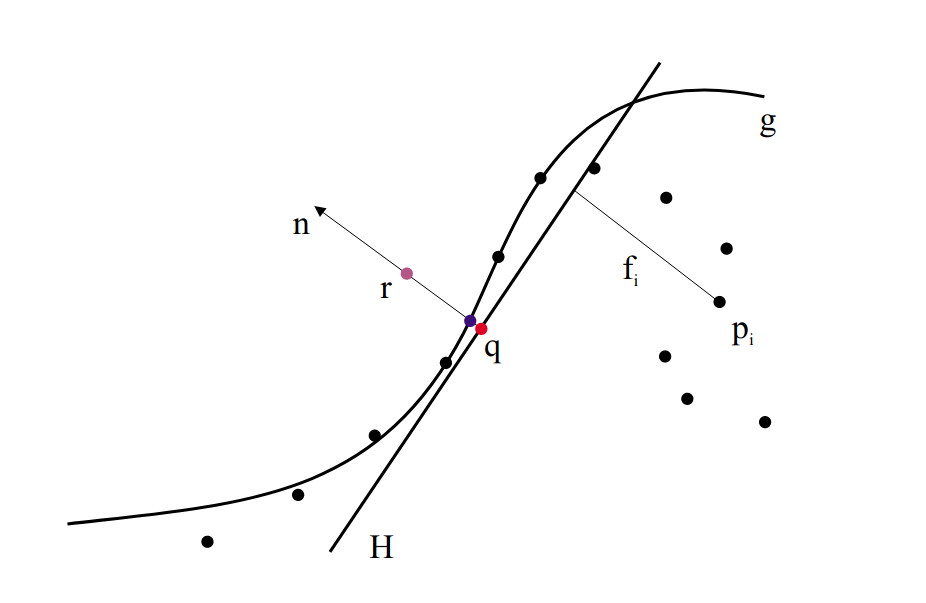
\includegraphics[scale=0.4]{0.png}


\section{Существующие алгоритмы}
\subsection{Оператор локально-оптимальной проекции(LOP)}
Происхождением метода является алгоритм Вайсфельда для решения задачи Ферма-Вебера о расположении точек, также известный как многомерная медиана L1. Это статистический инструмент, который традиционно применяется во всем мире для многомерных непараметрических точечных выборок, чтобы получить хороший представитель для большого количества выборок при наличии шума и выбросов. Проблема была впервые известна как проблема оптимального местоположения Вебера ~\cite{WEBER}. Задача состояла в том, чтобы найти оптимальное место для промплощадки, минимизирующее стоимость доступа. В статистике проблема известна как медиана L1 ~\cite{BROWN, SMALL}.

Задача Ферма-Вебера (глобальная) о расположении точек рассматривается как пространственная медиана, поскольку, будучи ограничена одномерным случаем, она совпадает с одномерной медианой и наследует некоторые ее свойства в многомерной постановке.

Реконструкция с помощью оператора проекции имеет важное достоинство: она определяет непротиворечивую геометрию на основе точек данных и предоставляет конструктивные средства для повышения ее дискретизации. 
Оператор локально-оптимальной проекции без параметризации использует более примитивный механизм проецирования, но поскольку он не основан на локальной 2D-параметризации, он более надежен и хорошо работает в сложных сценариях. Кроме того, если точки данных взяты локально с гладкой поверхности, оператор обеспечивает аппроксимацию второго порядка, что приводит к правдоподобной аппроксимации выбранной поверхности.

Оператор LOP имеет две непосредственные функции: во-первых, его можно использовать в качестве этапа предварительной обработки для любого другого метода реконструкции более высокого порядка (например, RBF). LOP можно применять к необработанным отсканированным данным для создания чистого набора данных, в качестве средства эффективного уменьшения шума и выбросов, а также для упрощения определения ориентации и топологии локальной поверхности. Во-вторых, его можно использовать для уточнения данного набора данных.

Для множества точек данных $P = \{p_j\}_{j\in J} \subset \mathbf R^{3}$, LOP проецирует произвольное множество точек $X^{(0)} = \{x_i^{(0)} \} _{i \in I} \subset \mathbf R^{3}$ на множество $P$, где $I$, $J$ обозначают наборы индексов. Множество спроецированных точек $Q = \{q_i\}_{i\in I}$ определяется так, чтобы оно минимизировало сумму взвешенных расстояний до точек P относительно радиальных весов с центром в том же множестве точек Q. Кроме того, точки Q не должны быть слишком близко друг к другу. Эта структура индуцирует определение искомых точек Q как решение уравнения с фиксированной точкой 
$$Q = G(Q),$$
где
$$G(C) = argmin_{X = \{x_i\}_{i \in I}} \{E_1(X,P,C) + E_2(X,C)\},$$
$$E_1(X,P,C) = \sum_{i \in I} \sum_{j \in J}\parallel x_i - p_j \parallel \theta(\parallel c_i - p_j \parallel), $$ 
$$E_2(X, C) = \sum _{i^{'} \in I} \lambda_{i^{'}}\sum_{i \in I \setminus\{i^{'}\}} \eta(\parallel x_{i^{'}}- c_i  \parallel)\theta(\parallel c_{i^{'}} - c_i \parallel)$$

Здесь $\theta(r)$ — быстро убывающая гладкая весовая функция с компактным опорным радиусом $h$, определяющая размер радиуса влияния, $\eta(r)$ — другая убывающая функция, штрафующая $x_{i^{'}}$ за то, что они подходят слишком близко к другим точкам, и $\{\lambda_i\}_{i \in I}$ являются уравновешивающими членами, которые обозначены через $\mathbf \land$. В двух словах, термин $E_1$ заставляет спроецированные точки $Q$ аппроксимировать геометрию $P$, а член $E_2$ стремится  сохранить справедливое распределение точек $Q$. Правильные значения $\mathbf\land$ могут гарантировать степень аппроксимации второго порядка оператора LOP при условии, что данные отбираются с поверхности $C^{2}$.


\section{Параллелизм}

Здесь будет параллельный алгоритм на псевдокоде




Параллельный алгоритм

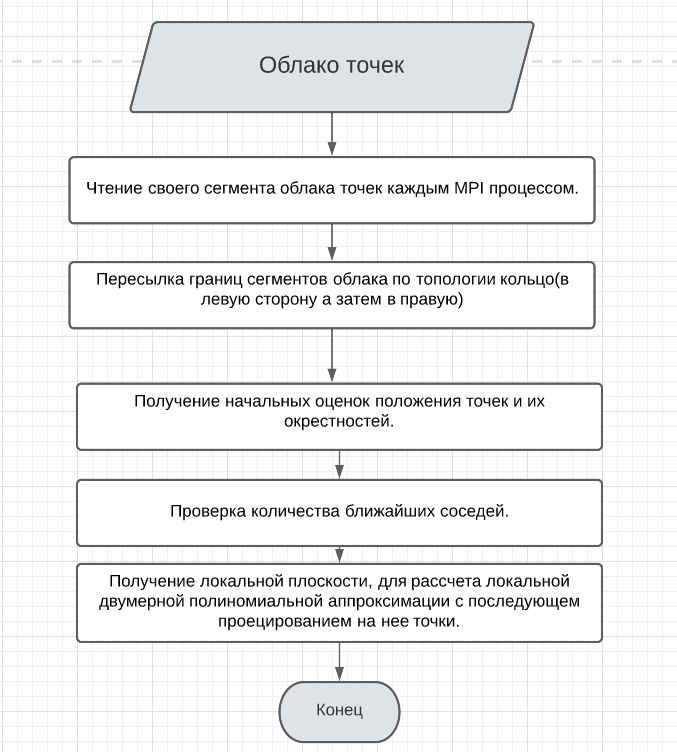
\includegraphics[scale=0.5]{1.png}

\section{Результаты экспериментов}

Время работы на n процессах n = 1...8


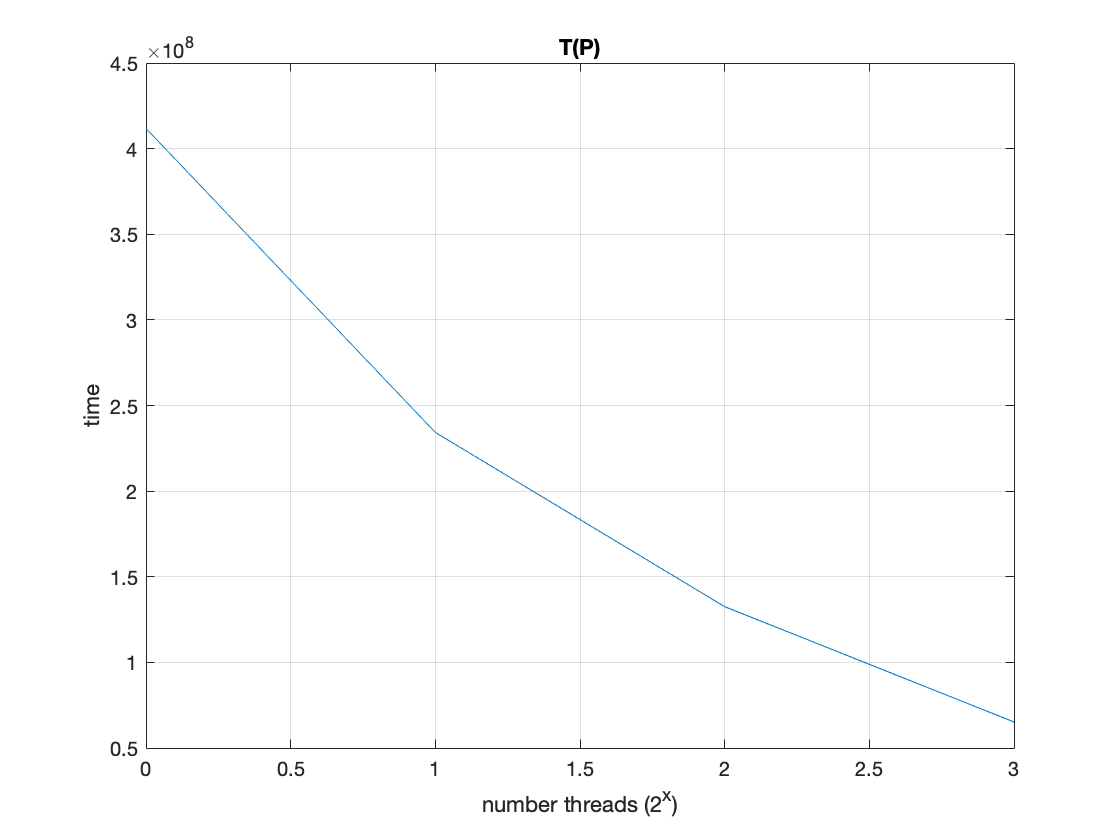
\includegraphics[scale=0.4]{T(P).png}

Ускорение:

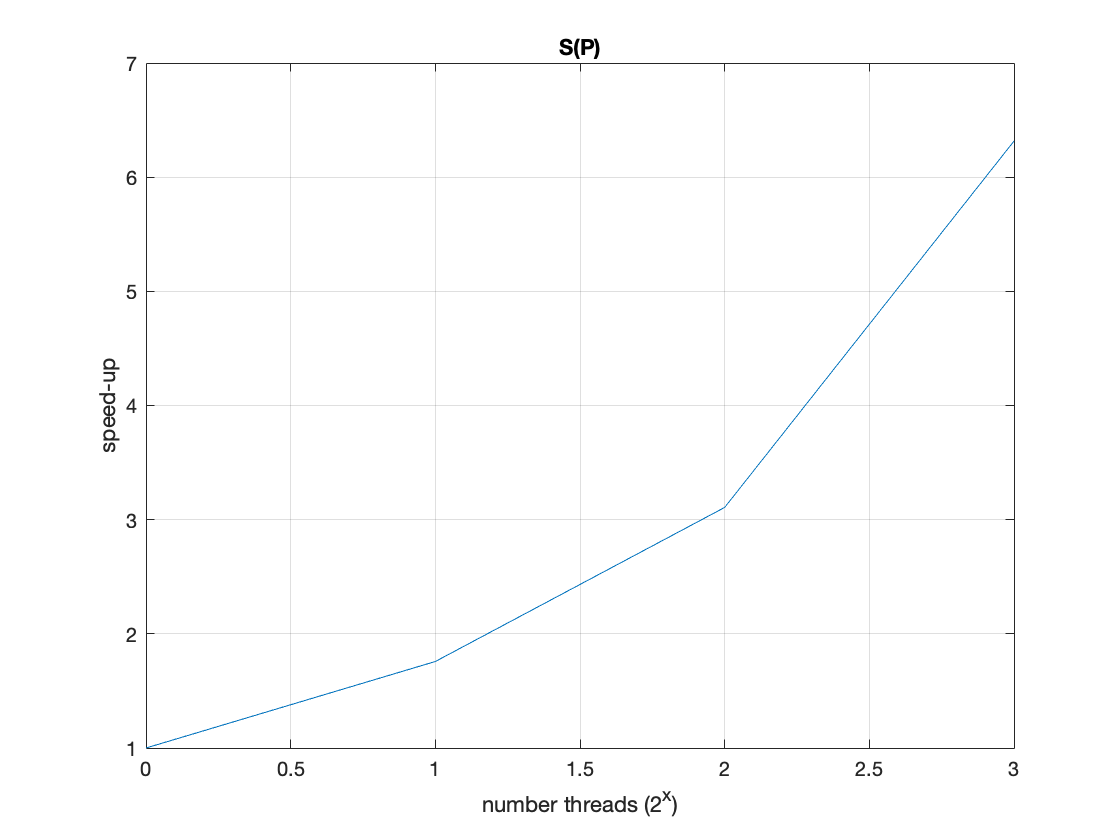
\includegraphics[scale=0.4]{S(P).png}

Эффективность:

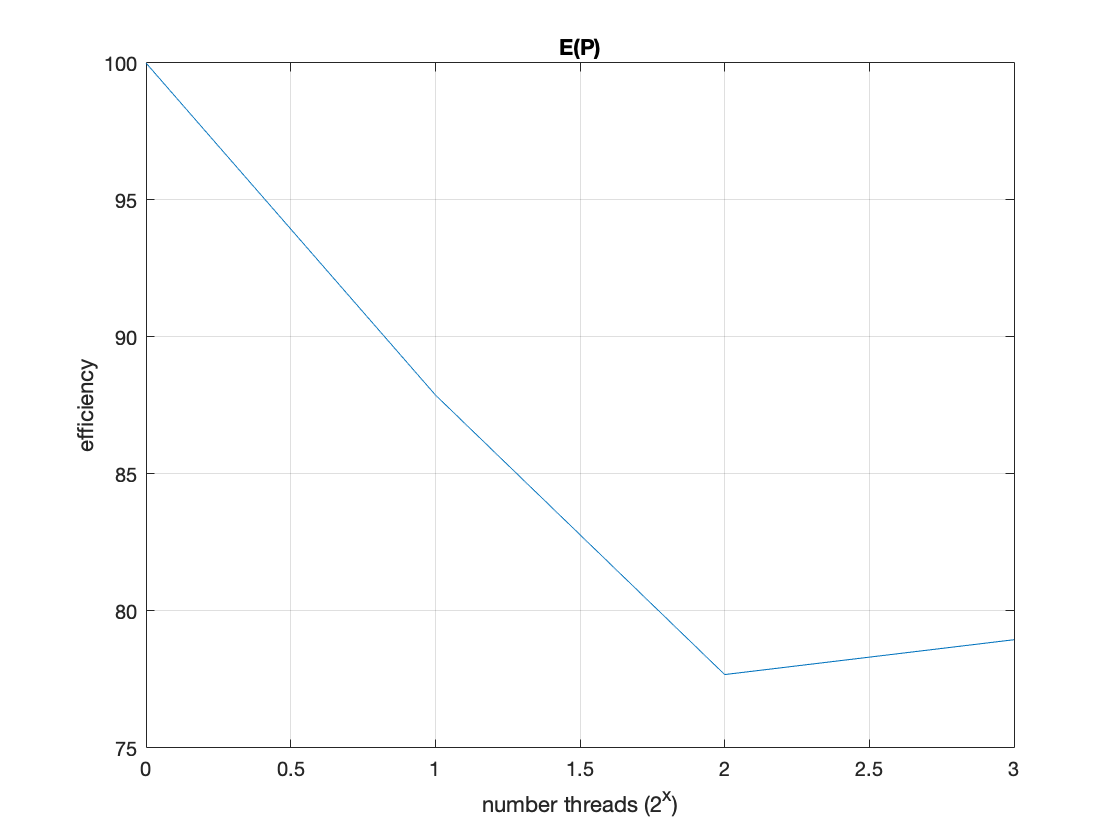
\includegraphics[scale=0.4]{E(P).png}

